\documentclass[tikz]{standalone}
\usetikzlibrary{positioning,shapes}
\begin{document}
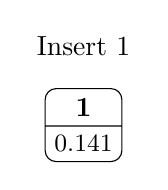
\begin{tikzpicture}[level 1/.style={sibling distance=12em},level 2/.style={sibling distance=7em},level 3/.style={sibling distance=4em},level 4/.style={sibling distance=2em},every node/.style = {draw, align=center, shape=rectangle split,rectangle split parts=2, rounded corners}]
\node(root) { \textbf{1}\nodepart{second}{\small 0.141}} ;
\node[shape=rectangle,draw=none,above of=root] {Insert 1};
\end{tikzpicture}
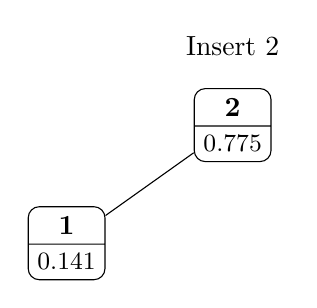
\begin{tikzpicture}[level 1/.style={sibling distance=12em},level 2/.style={sibling distance=7em},level 3/.style={sibling distance=4em},level 4/.style={sibling distance=2em},every node/.style = {draw, align=center, shape=rectangle split,rectangle split parts=2, rounded corners}]
\node(root) { \textbf{2}\nodepart{second}{\small 0.775}} 
child { node { \textbf{1}\nodepart{second}{\small 0.141}}  }
child[missing] {};
\node[shape=rectangle,draw=none,above of=root] {Insert 2};
\end{tikzpicture}
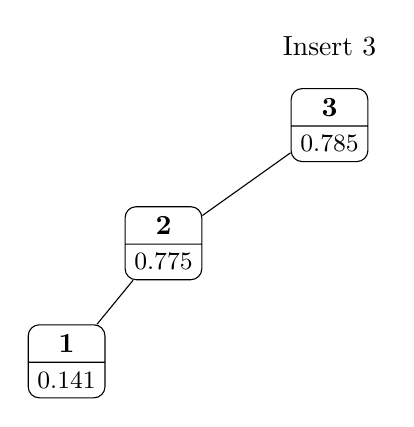
\begin{tikzpicture}[level 1/.style={sibling distance=12em},level 2/.style={sibling distance=7em},level 3/.style={sibling distance=4em},level 4/.style={sibling distance=2em},every node/.style = {draw, align=center, shape=rectangle split,rectangle split parts=2, rounded corners}]
\node(root) { \textbf{3}\nodepart{second}{\small 0.785}} 
child { node { \textbf{2}\nodepart{second}{\small 0.775}} 
child { node { \textbf{1}\nodepart{second}{\small 0.141}}  }
child[missing] {} }
child[missing] {};
\node[shape=rectangle,draw=none,above of=root] {Insert 3};
\end{tikzpicture}
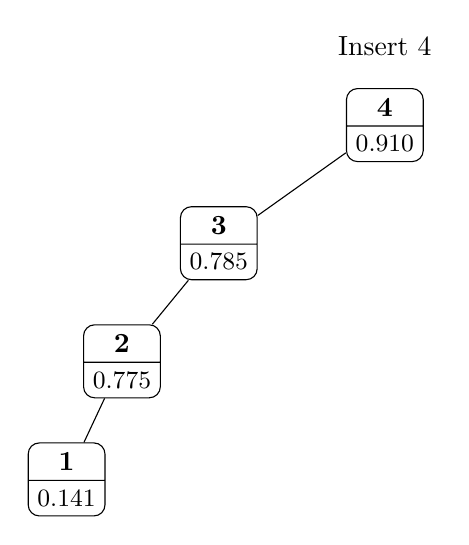
\begin{tikzpicture}[level 1/.style={sibling distance=12em},level 2/.style={sibling distance=7em},level 3/.style={sibling distance=4em},level 4/.style={sibling distance=2em},every node/.style = {draw, align=center, shape=rectangle split,rectangle split parts=2, rounded corners}]
\node(root) { \textbf{4}\nodepart{second}{\small 0.910}} 
child { node { \textbf{3}\nodepart{second}{\small 0.785}} 
child { node { \textbf{2}\nodepart{second}{\small 0.775}} 
child { node { \textbf{1}\nodepart{second}{\small 0.141}}  }
child[missing] {} }
child[missing] {} }
child[missing] {};
\node[shape=rectangle,draw=none,above of=root] {Insert 4};
\end{tikzpicture}
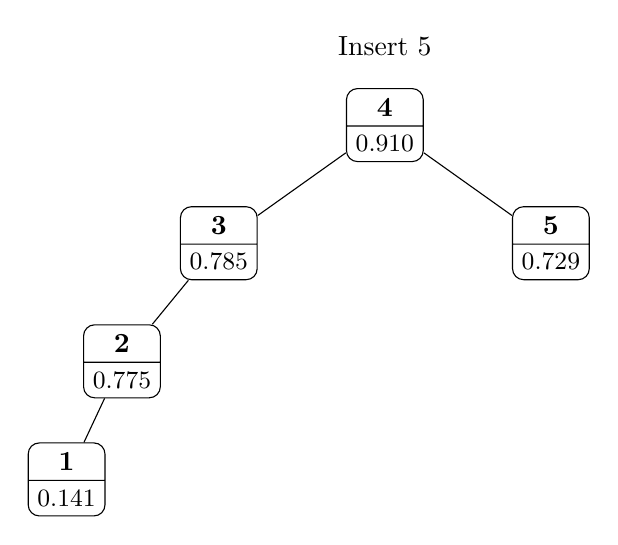
\begin{tikzpicture}[level 1/.style={sibling distance=12em},level 2/.style={sibling distance=7em},level 3/.style={sibling distance=4em},level 4/.style={sibling distance=2em},every node/.style = {draw, align=center, shape=rectangle split,rectangle split parts=2, rounded corners}]
\node(root) { \textbf{4}\nodepart{second}{\small 0.910}} 
child { node { \textbf{3}\nodepart{second}{\small 0.785}} 
child { node { \textbf{2}\nodepart{second}{\small 0.775}} 
child { node { \textbf{1}\nodepart{second}{\small 0.141}}  }
child[missing] {} }
child[missing] {} }
child { node { \textbf{5}\nodepart{second}{\small 0.729}}  };
\node[shape=rectangle,draw=none,above of=root] {Insert 5};
\end{tikzpicture}
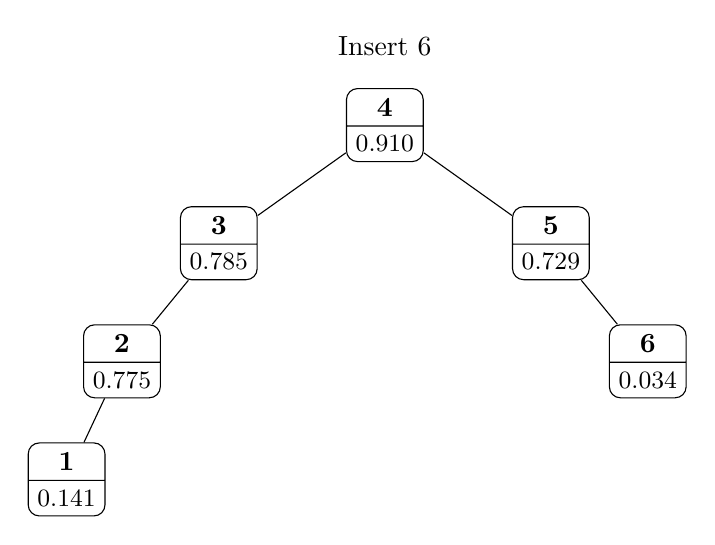
\begin{tikzpicture}[level 1/.style={sibling distance=12em},level 2/.style={sibling distance=7em},level 3/.style={sibling distance=4em},level 4/.style={sibling distance=2em},every node/.style = {draw, align=center, shape=rectangle split,rectangle split parts=2, rounded corners}]
\node(root) { \textbf{4}\nodepart{second}{\small 0.910}} 
child { node { \textbf{3}\nodepart{second}{\small 0.785}} 
child { node { \textbf{2}\nodepart{second}{\small 0.775}} 
child { node { \textbf{1}\nodepart{second}{\small 0.141}}  }
child[missing] {} }
child[missing] {} }
child { node { \textbf{5}\nodepart{second}{\small 0.729}} 
child[missing] {}
child { node { \textbf{6}\nodepart{second}{\small 0.034}}  } };
\node[shape=rectangle,draw=none,above of=root] {Insert 6};
\end{tikzpicture}
\begin{tikzpicture}
\node (b) {\begin{tikzpicture}[level 1/.style={sibling distance=12em},level 2/.style={sibling distance=7em},level 3/.style={sibling distance=4em},level 4/.style={sibling distance=2em},every node/.style = {draw, align=center, shape=rectangle split,rectangle split parts=2, rounded corners}]
\node(root) { \textbf{4}\nodepart{second}{\small 0.910}} 
child[missing] {}
child { node { \textbf{5}\nodepart{second}{\small 0.729}}  };
\end{tikzpicture}
};
\node[left=of b] {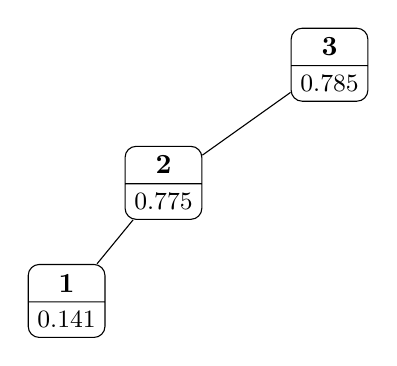
\begin{tikzpicture}[level 1/.style={sibling distance=12em},level 2/.style={sibling distance=7em},level 3/.style={sibling distance=4em},level 4/.style={sibling distance=2em},every node/.style = {draw, align=center, shape=rectangle split,rectangle split parts=2, rounded corners}]
\node(root) { \textbf{3}\nodepart{second}{\small 0.785}} 
child { node { \textbf{2}\nodepart{second}{\small 0.775}} 
child { node { \textbf{1}\nodepart{second}{\small 0.141}}  }
child[missing] {} }
child[missing] {};
\end{tikzpicture}
};
\node[right=of b] {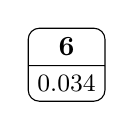
\begin{tikzpicture}[level 1/.style={sibling distance=12em},level 2/.style={sibling distance=7em},level 3/.style={sibling distance=4em},level 4/.style={sibling distance=2em},every node/.style = {draw, align=center, shape=rectangle split,rectangle split parts=2, rounded corners}]
\node(root) { \textbf{6}\nodepart{second}{\small 0.034}} ;
\end{tikzpicture}
};
\node[above=of b] {Move [4, 5] to start};
\node[below=of b] {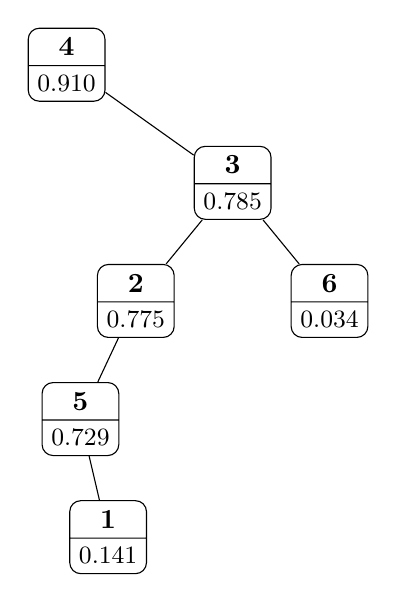
\begin{tikzpicture}[level 1/.style={sibling distance=12em},level 2/.style={sibling distance=7em},level 3/.style={sibling distance=4em},level 4/.style={sibling distance=2em},every node/.style = {draw, align=center, shape=rectangle split,rectangle split parts=2, rounded corners}]
\node(root) { \textbf{4}\nodepart{second}{\small 0.910}} 
child[missing] {}
child { node { \textbf{3}\nodepart{second}{\small 0.785}} 
child { node { \textbf{2}\nodepart{second}{\small 0.775}} 
child { node { \textbf{5}\nodepart{second}{\small 0.729}} 
child[missing] {}
child { node { \textbf{1}\nodepart{second}{\small 0.141}}  } }
child[missing] {} }
child { node { \textbf{6}\nodepart{second}{\small 0.034}}  } };
\end{tikzpicture}
};
\end{tikzpicture}
\begin{tikzpicture}
\node (b) {\begin{tikzpicture}[level 1/.style={sibling distance=12em},level 2/.style={sibling distance=7em},level 3/.style={sibling distance=4em},level 4/.style={sibling distance=2em},every node/.style = {draw, align=center, shape=rectangle split,rectangle split parts=2, rounded corners}]
\node(root) { \textbf{2}\nodepart{second}{\small 0.775}} 
child { node { \textbf{1}\nodepart{second}{\small 0.141}}  }
child[missing] {};
\end{tikzpicture}
};
\node[left=of b] {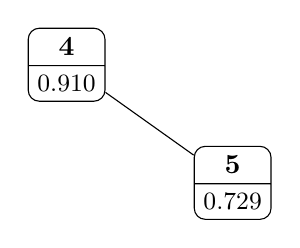
\begin{tikzpicture}[level 1/.style={sibling distance=12em},level 2/.style={sibling distance=7em},level 3/.style={sibling distance=4em},level 4/.style={sibling distance=2em},every node/.style = {draw, align=center, shape=rectangle split,rectangle split parts=2, rounded corners}]
\node(root) { \textbf{4}\nodepart{second}{\small 0.910}} 
child[missing] {}
child { node { \textbf{5}\nodepart{second}{\small 0.729}}  };
\end{tikzpicture}
};
\node[right=of b] {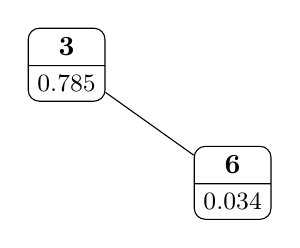
\begin{tikzpicture}[level 1/.style={sibling distance=12em},level 2/.style={sibling distance=7em},level 3/.style={sibling distance=4em},level 4/.style={sibling distance=2em},every node/.style = {draw, align=center, shape=rectangle split,rectangle split parts=2, rounded corners}]
\node(root) { \textbf{3}\nodepart{second}{\small 0.785}} 
child[missing] {}
child { node { \textbf{6}\nodepart{second}{\small 0.034}}  };
\end{tikzpicture}
};
\node[above=of b] {Move [3, 4] to start};
\node[below=of b] {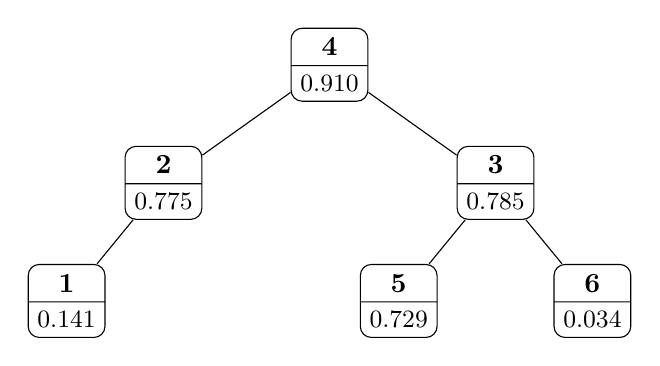
\begin{tikzpicture}[level 1/.style={sibling distance=12em},level 2/.style={sibling distance=7em},level 3/.style={sibling distance=4em},level 4/.style={sibling distance=2em},every node/.style = {draw, align=center, shape=rectangle split,rectangle split parts=2, rounded corners}]
\node(root) { \textbf{4}\nodepart{second}{\small 0.910}} 
child { node { \textbf{2}\nodepart{second}{\small 0.775}} 
child { node { \textbf{1}\nodepart{second}{\small 0.141}}  }
child[missing] {} }
child { node { \textbf{3}\nodepart{second}{\small 0.785}} 
child { node { \textbf{5}\nodepart{second}{\small 0.729}}  }
child { node { \textbf{6}\nodepart{second}{\small 0.034}}  } };
\end{tikzpicture}
};
\end{tikzpicture}
\begin{tikzpicture}
\node (b) {\begin{tikzpicture}[level 1/.style={sibling distance=12em},level 2/.style={sibling distance=7em},level 3/.style={sibling distance=4em},level 4/.style={sibling distance=2em},every node/.style = {draw, align=center, shape=rectangle split,rectangle split parts=2, rounded corners}]
\node(root) { \textbf{4}\nodepart{second}{\small 0.910}} 
child { node { \textbf{2}\nodepart{second}{\small 0.775}}  }
child[missing] {};
\end{tikzpicture}
};
\node[left=of b] {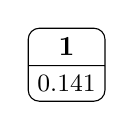
\begin{tikzpicture}[level 1/.style={sibling distance=12em},level 2/.style={sibling distance=7em},level 3/.style={sibling distance=4em},level 4/.style={sibling distance=2em},every node/.style = {draw, align=center, shape=rectangle split,rectangle split parts=2, rounded corners}]
\node(root) { \textbf{1}\nodepart{second}{\small 0.141}} ;
\end{tikzpicture}
};
\node[right=of b] {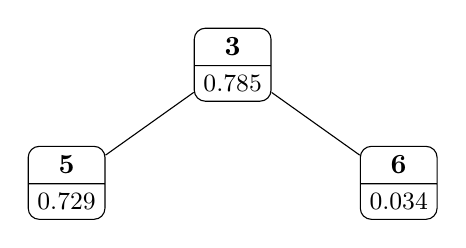
\begin{tikzpicture}[level 1/.style={sibling distance=12em},level 2/.style={sibling distance=7em},level 3/.style={sibling distance=4em},level 4/.style={sibling distance=2em},every node/.style = {draw, align=center, shape=rectangle split,rectangle split parts=2, rounded corners}]
\node(root) { \textbf{3}\nodepart{second}{\small 0.785}} 
child { node { \textbf{5}\nodepart{second}{\small 0.729}}  }
child { node { \textbf{6}\nodepart{second}{\small 0.034}}  };
\end{tikzpicture}
};
\node[above=of b] {Move [2, 3] to start};
\node[below=of b] {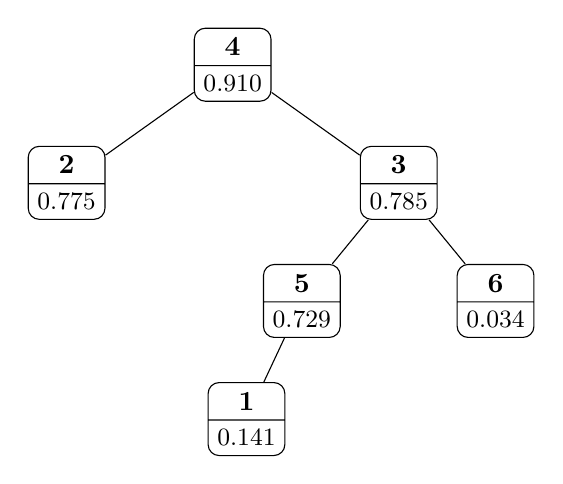
\begin{tikzpicture}[level 1/.style={sibling distance=12em},level 2/.style={sibling distance=7em},level 3/.style={sibling distance=4em},level 4/.style={sibling distance=2em},every node/.style = {draw, align=center, shape=rectangle split,rectangle split parts=2, rounded corners}]
\node(root) { \textbf{4}\nodepart{second}{\small 0.910}} 
child { node { \textbf{2}\nodepart{second}{\small 0.775}}  }
child { node { \textbf{3}\nodepart{second}{\small 0.785}} 
child { node { \textbf{5}\nodepart{second}{\small 0.729}} 
child { node { \textbf{1}\nodepart{second}{\small 0.141}}  }
child[missing] {} }
child { node { \textbf{6}\nodepart{second}{\small 0.034}}  } };
\end{tikzpicture}
};
\end{tikzpicture}
\end{document}
